\chapter{Interfacing a DC Motor}
\thispagestyle{empty}
\label{dcmotor}
\newcommand{\LocDCMfig}{\Origin/user-code/dcmotor/figures}
\newcommand{\LocDCMscicode}{\Origin/user-code/dcmotor/scilab}
\newcommand{\LocDCMscibrief}[1]{{\tt \seqsplit{
        Origin/user-code/dcmotor/scilab/#1}},
  see \fnrefp{fn:file-loc}}
\newcommand{\LocDCMardcode}{\Origin/user-code/dcmotor/arduino}
\newcommand{\LocDCMardbrief}[1]{{\tt \seqsplit{
        Origin/user-code/dcmotor/arduino/#1}},
  see \fnrefp{fn:file-loc}}

%%%%%%%%%%%%%python starts
\newcommand{\LocDCMpycode}{\Origin/user-code/dcmotor/python}
\newcommand{\LocDCMpybrief}[1]{{\tt \seqsplit{
        Origin/user-code/dcmotor/python/#1}},
  see \fnrefp{fn:file-loc}}
%%%%%%%%%%%%%python ends

%%%%%%%%%%%%%julia starts
\newcommand{\LocDCMjuliacode}{\Origin/user-code/dcmotor/julia}
\newcommand{\LocDCMjuliabrief}[1]{{\tt \seqsplit{
        Origin/user-code/dcmotor/julia/#1}},
  see \fnrefp{fn:file-loc}}
%%%%%%%%%%%%%julia ends

%%%%%%OpenModelica Starts
\newcommand{\LocDCMOpenModelicacode}{\Origin/user-code/dcmotor/OpenModelica}  %added for OpenModelica
\newcommand{\LocDCMOpenModelicabrief}[1]{{\tt \seqsplit{%
        Origin/user-code/led/OpenModelica/#1}}, see \fnrefp{fn:file-loc}} % added for OpenModelica

%%%%%OpenModelcia Ends

Motors are widely used in commercial applications. 
DC motor converts electric power obtained from direct current to 
mechanical motion. This chapter describes the experiments to 
control DC motor with \arduino\ board. We will observe the 
direction of motion of the DC motor being changed 
using the microcontroller on \arduino\ board. 
Control instruction will be sent to \arduino\ using Arduino IDE, 
Scilab scripts, Scilab Xcos, Python, Julia, and OpenModelica. 
The experiments provided in this chapter don't require the shield. 
Therefore, the readers must remove the shield from the \arduino\ before 
moving further in this chapter. Before removing the shield, 
the readers are advised to detach \arduino\ from the computer. 

\section{Preliminaries}
In order to change its direction, the sign of the voltage applied to
the DC motor is changed.  For that, one needs to use external hardware
called \index{H-Bridge circuit DC motor}%
H-Bridge circuit DC motor with \arduino. \index{H-Bridge}%
H-Bridge allows direction of the current passing through the DC motor
to be changed. It avoids the sudden short that may happen while
changing the direction of current passing through the motor.  It is
one of the essential circuits for the smooth operation of a DC
motor. There are many manufacturers of H-bridge circuit viz.
\index{L293D,L298}%
L293D, L298, etc.  Often they provide small \index{PCB breakout
  board}%
PCB breakout boards.  These modules also provide an extra supply that
is needed to drive the DC motor.  \figref{fig:motordriverboard} shows
the diagram of a typical breakout board containing IC L293D, which will
be used in this book. One may note that the toolboxes presented in this book supports three types of H-Bridge circuit. \tabref{table:convention} provides the values to be passed for different H-Bridge circuits. \par

\begin{figure}
  \centering
  \includegraphics[width=\lgfig]{\LocDCMfig/dcmotor_board.png}
  \caption{L293D motor driver board}
  \label{fig:motordriverboard}
\end{figure}

\begin{table}
  \centering
  \caption{Values in the \scilab\ command for different H-Bridge circuits}
  \label{table:convention}
  \begin{tabular}{llc}\hline
    Type of H-Bridge circuit & Value \\ \hline
    MotorShield Rev3         & 1     \\ \hline 
    PMODHB5/L298             & 2     \\ \hline 
    L293D                    & 3     \\ \hline
  \end{tabular}
\end{table}

Input from \arduino\ to H-bridge IC is in \index{pulse width
  modulation, PWM}%
pulse width modulation (PWM) form. PWM is a technique to generate
analog voltages using digital pins. We know that \arduino\ has digital
input-output pins. When these pins are configured as an output, they
provide High (5V) or Low (0V) voltage. With PWM technique, these pins
are switched on and off iteratively and fast enough so that the
voltage is averaged out to some analog value in between 0-5V. This
analog value depends on ''switch-on'' time and ''switch-off''
time. For example, if both ''switch-on'' time and ''switch-off'' time
are equal, average voltage on PWM pin will be 2.5V. To enable fast
switching of digital pin, a special hardware is provided in
microcontrollers.  PWM is considered as an important resource of
the microcontroller system. \arduino\ board has 6 PWM pins (3, 5, 6, 9, 10, 11) \cite{arduino-pwm}. 
On an original \arduino\ board, these pins are marked with a tilde sign next to the pin number, 
as shown in \figref{fig:uno-pwm}. For each of these pins, the input can come from 8 bits.
Thus we can generate $2^8 = 256$ different analog values (from 0 to 255) 
in between 0-5V with these pins.

\begin{figure}
  \centering
  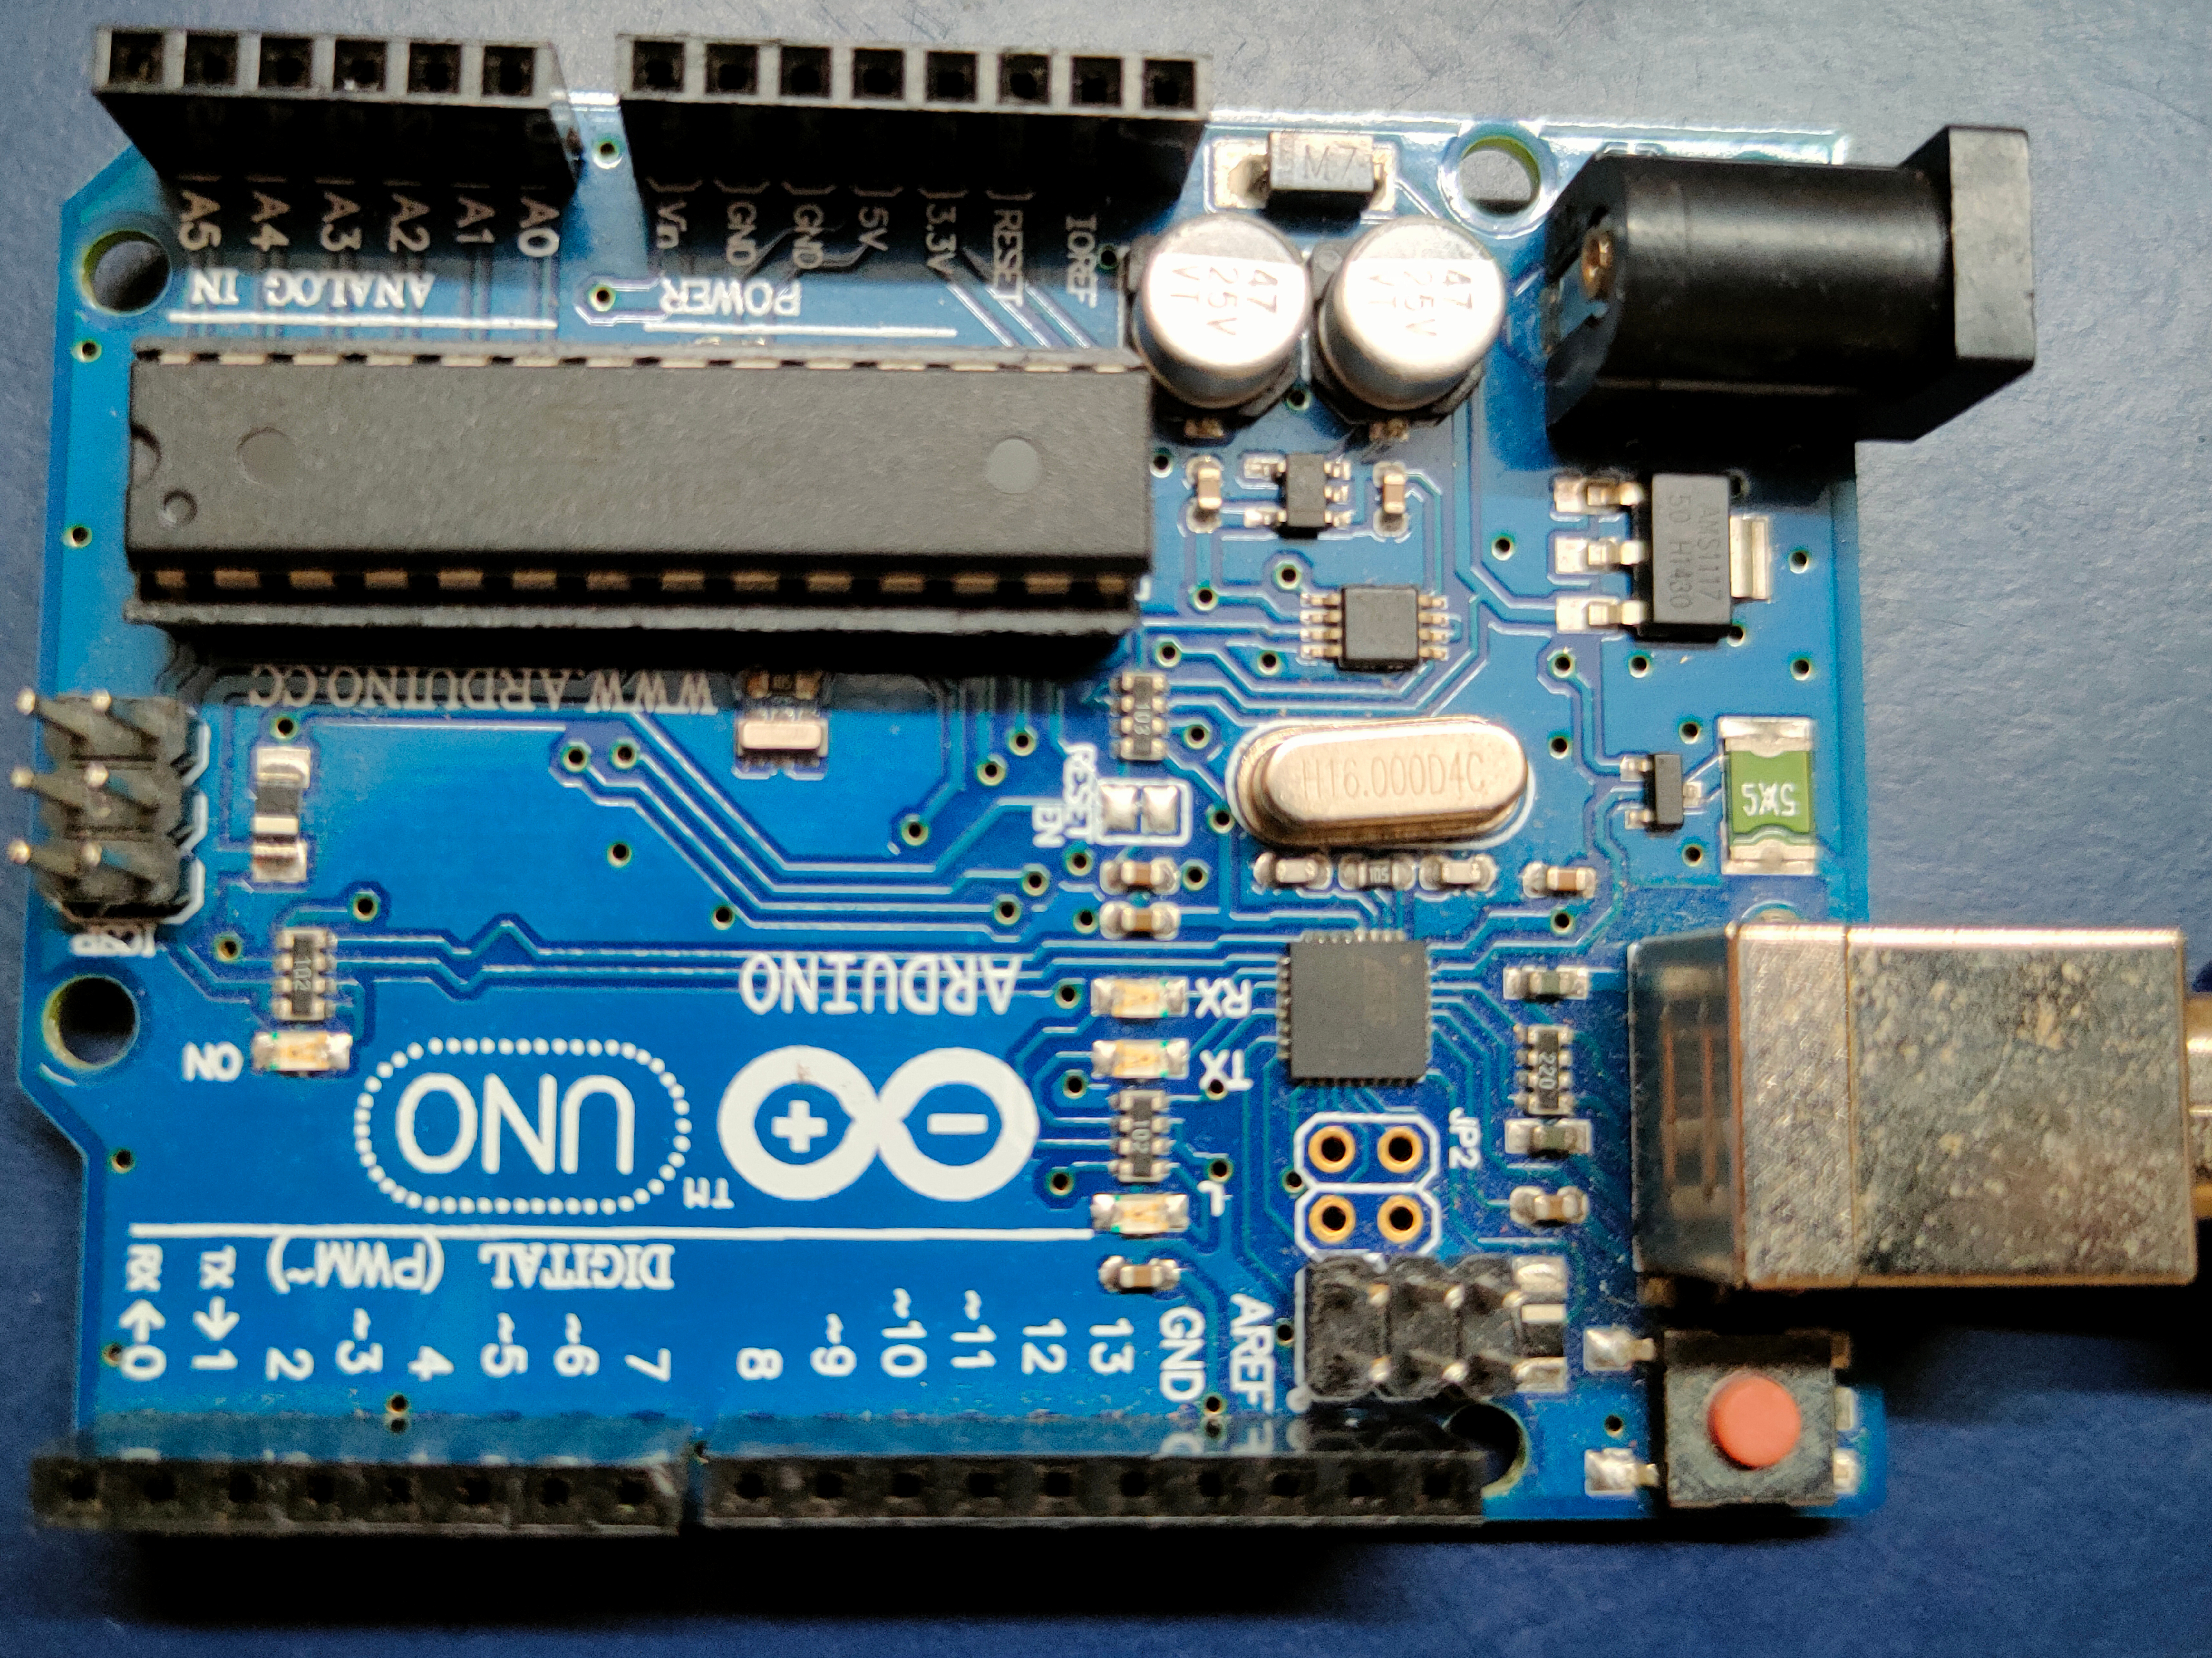
\includegraphics[width=\lgfig]{\LocDCMfig/uno-pwm.jpg}
  \caption{PWM pins on an \arduino\ board}
  \label{fig:uno-pwm}
\end{figure}

We now carry out the following connections:
\begin{enumerate}
  \item Connect input of L293D (M1\_IN) pins to two of the PWM pins
        available on \arduino.  We have used pins 9 and 10 of the \arduino\
        board. 
  \item Connect the output of the L293D (M1\_OUT) pins directly to the 2
        wires of the DC motor.  As the direction is changed during the
        operation, the polarity of the connection does not matter.
  \item Connect supply (Vcc) and ground (Gnd) pins of L293D to 5V and
        Gnd pins of the \arduino\ board, respectively.
\end{enumerate}
A schematic of these connections is given in
\figref{fig:dcm-schematic}.  The actual connections can be seen in
\figref{fig:dcmotorconn}.


\begin{figure}
  \centering
  \includegraphics[width=\smfig]{\LocDCMfig/schematic.png}
  \caption{A schematic of DC motor connections}
  \label{fig:dcm-schematic}
\end{figure}
\begin{figure}
  \centering
  \includegraphics[width=\lgfig]{\LocDCMfig/dc_motor_description.jpg}
  \caption{How to connect the DC motor to the \arduino\ board}
  \label{fig:dcmotorconn}
\end{figure}

\section{Controlling the DC motor from Arduino}
\subsection{Controlling the DC motor}
\label{sec:dcm-ard}
In this section, we will describe some experiments that will help
drive the DC motor from the Arduino IDE.  We will also give the
necessary code.  We will present three experiments in this section. 
As mentioned earlier, the shield must be removed from 
the \arduino\ and the \arduino\ needs to be connected to the computer 
with a USB cable, as shown in \figref{arduino}. The reader should go through the
instructions given in \secref{sec:ard-start} before getting started. 

\paragraph{Note:} The readers are advised to affix a small 
(very lightweight) piece of paper at the tip of the shaft of the DC motor. 
That will help them observe the direction of rotation 
of the DC motor while running the experiments. 

\begin{enumerate}
  \item We now demonstrate how to drive the DC motor from the Arduino
        IDE.  \ardref{ard:dcmotor-clock} has the required code for this.  It
        starts the serial port at a baud rate of 115200.  Pins 9 and 10 are
        declared as output pins and hence values can be written on to them. The following 
        lines are used to declare these two pins as output pins: 
        \lstinputlisting[firstline=3,lastline=4]
        {\LocDCMardcode/dcmotor-clock/dcmotor-clock.ino}
        Next, we write PWM 100 on pin 9 and PWM 0 on pin 10, as shown below:
        \lstinputlisting[firstline=5,lastline=6]
        {\LocDCMardcode/dcmotor-clock/dcmotor-clock.ino}
        Recall from \figref{fig:dcmotorconn} that pins 9 and 10 are connected to the
        input of the breakout board, which in turn makes the DC motor run at
        an intermediate speed.  Some of the breakout boards may not have enough current driving
        capability and hence tend to heat up.  To avoid these difficulties,
        the DC motor is run at an intermediate value of PWM 100. Remember, we can 
        increase this value upto 255. 
        % As mentioned in \secref{sec:led-pril}, a high on pin 9 also makes the blue LED turn on. 
        
        The line containing {\tt delay} makes the previous command execute
        for 3 seconds.  As a result, the DC motor continues to rotate for 3
        seconds.  After this, we put a 0 in both pins 9 and 10, as shown below:
        \lstinputlisting[firstline=8,lastline=9]
        {\LocDCMardcode/dcmotor-clock/dcmotor-clock.ino}
        With this, the motor comes to a halt.  
        % The blue LED is also turned off.
        
  \item It is easy to make the DC motor run in the reverse direction by
        interchanging the values put on pins 9 and 10.  This is done in
        \ardref{ard:dcmotor-both}.  In this code, we make the DC motor
        run in one direction for 3 seconds and then make it rotate in the
        reverse direction for 2 seconds.  The rotation in reverse direction
        is achieved by putting 100 in pin 10, as shown below:
        \lstinputlisting[firstline=8,lastline=9]
        {\LocDCMardcode/dcmotor-both/dcmotor-both.ino}
        % This makes the green LED light up as well, recall the discussion in \secref{sec:led-pril}.  After
        Next, we release the motor by writing 0 in both pins 9 and 10, as shown below:
        \lstinputlisting[firstline=11,lastline=12]
        {\LocDCMardcode/dcmotor-both/dcmotor-both.ino}
        With this, the motor comes to a halt.  
        % This turns the green LED off as well.
        
  \item Next, we make the DC motor run in forward and reverse
        directions, in a loop.  This is done through
        \ardref{ard:dcmotor-loop}.  We first write PWM 100 in pin 9 for 3
        seconds.  After that, make the motor stop for 2 seconds.  Finally,
        make the motor rotate in the reverse direction by writing PWM 100 in pin 10
        for two seconds.  Finally, we make the motor stop for one second.
        The entire thing is put in a {\tt for} loop which runs for 5 iterations. 
\end{enumerate}

\begin{exercise}
  Carry out the following exercise:
  \begin{enumerate}
    \item Try out some of the suggestions given above, \ie\ removing
          certain numbers from the code
    \item See if the DC motor runs if you put 1 instead of 100 as the PWM
          value.  Explain why it does not run.  Find out the smallest value at
          which it will start running.
  \end{enumerate}
\end{exercise}

\subsection{Arduino Code}
\label{sec:dcmotor-arduino-code}
\lstset{style=mystyle}
\addtocontents{ard}{\protect\addvspace{\codclr}}

\begin{ardcode}
  \acaption{Rotating the DC motor}
  {Rotating the DC motor.  Available at
    \LocDCMardbrief{dcmotor-clock/dcmotor-clock.ino}.}
  \label{ard:dcmotor-clock}
  \lstinputlisting{\LocDCMardcode/dcmotor-clock/dcmotor-clock.ino}
\end{ardcode}

\begin{ardcode}
  \acaption{Rotating the DC motor in both directions}{Rotating the DC
    motor in both directions.  
    Available at
    \LocDCMardbrief{dcmotor-both/dcmotor-both.ino}.}
  \label{ard:dcmotor-both}
  \lstinputlisting{\LocDCMardcode/dcmotor-both/dcmotor-both.ino}
\end{ardcode}

\begin{ardcode}
  \acaption{Rotating the DC motor in both directions in a loop}{Rotating
    the DC motor in both directions in a loop.
    Available at
    \LocDCMardbrief{dcmotor-loop/dcmotor-loop.ino}.}
  \label{ard:dcmotor-loop}
  \lstinputlisting{\LocDCMardcode/dcmotor-loop/dcmotor-loop.ino}
\end{ardcode}


